\documentclass[11pt,a4paper]{article}
\usepackage[T1]{fontenc}
\usepackage{graphicx}
\usepackage{amssymb}
\usepackage{xcolor}
\usepackage[hidelinks,colorlinks=true,urlcolor=blue,linkcolor=teal]{hyperref}
\usepackage{minted}
\usepackage[margin=1in]{geometry}
% \usepackage{longtable}
\usepackage{setspace}
\usepackage{mathtools}
\usepackage{makecell}
\usepackage[most]{tcolorbox}
\usepackage{float}
\usepackage{titlesec}
\usepackage{datetime2}
\usepackage{caption}

\tcbset{enhanced,colback=white,colframe=cyan!75!black,fonttitle=\bfseries}
\hypersetup{
	pdftitle={DSP Lab solved problems},
	pdfsubject={Solution to problems created from Gemini}
}

\newcommand{\note}[1]{%
	\begin{tcolorbox}[colframe=orange!75!black]
		#1
	\end{tcolorbox}
}
\newcommand{\importMLCode}[1]{%
	\setstretch{1}
	\inputminted[autogobble]{matlab}{#1}
	\setstretch{1.15}
}
\newcommand{\inc}[1]{\includegraphics[width=\textwidth]{img/#1}}

% \renewcommand\cellgape{\Gape[10pt]}

\begin{document}
\setstretch{1.15}
\begin{center}
	{\Huge \normalfont \underline{DSP Lab Solved problems}}
	
	\vspace*{10pt}
	\texttt{Last updated: \today\ \DTMcurrenttime}
	
	\href{https://github.com/roopeshor/tex-works/tree/main/Lab\%20Programs/DSP}{\LaTeX\ source here}
	\vspace*{10pt}
\end{center}
% \titleformat{\section}[display]{}{}{}{\bfseries\huge\filcenter}
% \titlespacing{\section}{0pt}{10pt}{20pt}
\pagenumbering{gobble}
\note{I asked Gemini to create some problems for me. And these are solution to some of them.}
\begin{center}
	{\let\clearpage\relax \tableofcontents}
\end{center}

% \vspace*{20pt}
% \note{These are notes I made along while I was studying for exam (and later refined).
% Many implementations done here are directly based on the theory. Hence certain things might be confusing at first.
% This is intended as a reference, and defintly not something to mug up at a night before exam. :)

% Also in each program I've put plotting codes inside a function (such as \mintinline{matlab}|plot_sig_fft|, \mintinline{matlab}|plot_|, \texttt{stairz}, etc..)
% This is to make code look neater, so that logic of program is not much obstructed by code to plot things
% }

% \titleformat{\section}[frame]
% {\pagebreak \Large\fontfamily{qpl}\selectfont}
% {\filcenter\enspace \thesection\enspace}
% {10pt} % margin-bottom
% {\filcenter}
% \pagebreak
\pagenumbering{arabic}
\setlength{\parindent}{0pt}
\section{FIR Filter Design for Signal Restoration}

You are given a discrete-time signal $x(n)$ which is a combination of a desired low-frequency signal and an unwanted high-frequency noise component. The signal is defined as:

$$x(n)=\cos(0.1\pi n)+0.5sin(0.8\pi n)\quad \text{for} 0\le n\le 100$$
Question is:
\begin{enumerate}
	\item Design a digital FIR low-pass filter to remove the high-frequency noise component.
	\item Filter the input signal using designed filter
\end{enumerate}

\subsection*{Program}
\importMLCode{code/Q1.m}
\begin{figure*}[h!]
	\begin{minipage}{.45\textwidth}
		\caption*{Plotted signal}
		\inc{Q11.pdf}
		\vspace*{10pt}
		\caption*{Filter's frequency response}
		\inc{Q12.pdf}
	\end{minipage}%
	\hfill%
	\begin{minipage}{.45\textwidth}
		\caption*{Input message spectrum}
		\inc{Q13.pdf}
		\vspace*{10pt}
		\caption*{Filtered Output spectrum}
		\inc{Q14.pdf}
	\end{minipage}
\end{figure*}
\section{LTI System Stability Analysis and Modification}
Consider the LTI system described by the following difference equation:

$$y(n)-1.2y(n-1)+0.8y(n-2)=x(n)$$

Question:

\begin{enumerate}
	\item Determine if this system is stable or not
	\item Plot poles and zeros of the system
	\item Compute and plot the impulse response of the system for $0\le n\le 50$
	\item Modify the system by changing the coefficient of $y(n-1)$ and $y(n-2)$ so that the poles are located at $p=0.5\pm 0.5j$. Plot the pole-zero diagram for new system
\end{enumerate}

\subsection*{Program for Question 1-3:}

\importMLCode{code/Q21.m}


\begin{figure*}[ht!]
	\begin{minipage}{.45\textwidth}
		\inc{Q21.pdf}
	\end{minipage}%
	\hfill%
	\begin{minipage}{.45\textwidth}
		\inc{Q22.pdf}
	\end{minipage}
\end{figure*}

\hrule
\subsection*{Program For Question 4}
\vspace*{10pt}

Given system has 2 zeros at $p = 0$ and 2 poles. To change the poles location to $p=0.5\pm 0.5j$, First write it in system function form, change denominator expressions and work backwards: (here $z^2$ implies double zero at $p = 0$)
\begin{align*}
	H'(z) &= \frac{z^2}{(z - p_1)(z - p_2)}\\
	H'(z) &= \frac{z^2}{
		\left[z - \left(0.5 + 0.5i\right)\right]
		\left[z - \left(0.5 - 0.5i\right)\right]
	} \\
	 &= \frac{z^2}{z^2 -1z + 0.5} \\
	 \frac{Y(z)}{X(z)} &= \frac{1}{1 -1z^{-1} + 0.5z^{-2}} \\
	 \Rightarrow X(z) &= Y(z)\left[1 -1z^{-1} + 0.5z^{-2}\right]
\end{align*}

Applying inverse Z-transform gives the required system:
$$x(n) = y(n) - y(n - 1) + 0.5y(n - 2)$$
Hence the implementation: 
\importMLCode{code/Q22.m}
\begin{figure*}[ht!]
	\centering
	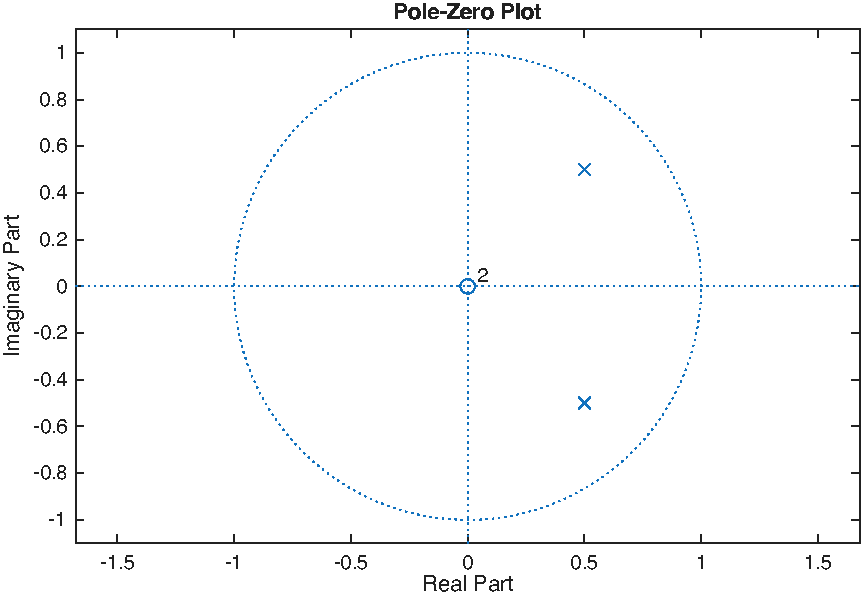
\includegraphics[width=.5\textwidth]{img/Q23.pdf}
	\caption*{new system function}
\end{figure*}
\pagebreak
\section{Simulation of Gibbs oscillation}
Simulate Gibbs oscillation on a given signal $s(t) = \text{sgn}(t)$.

\subsection*{Background}
The Fourier series of a complex-valued periodic function $s(t)$, integrable over the interval $[a, b]$on the real line, is defined as: 
$$s(t) = \sum _{n=-\infty }^{\infty }c_{n}e^{i2\pi {\tfrac {n}{T}}t}$$

Where $T = b - a$ is the period of function. Fourier coefficients $c_{n}$ are: 
$$c_{n}={\frac {1}{T}}\int _{a}^{b}s(t)\ e^{-i2\pi {\tfrac {n}{T}}t}dt$$


\subsection*{Program}
\importMLCode{code/Q4.m}

\begin{figure*}[ht!]
	\centering
	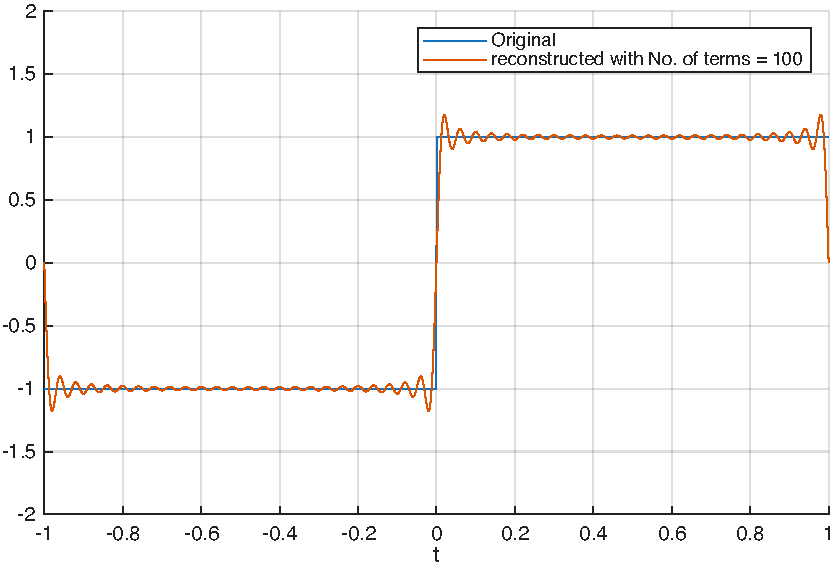
\includegraphics[width=.5\textwidth]{img/Q4.pdf}
	\caption*{Notice the wide oscillation near discontinuities}
\end{figure*}
\section{Extraction of periodic signals from noisy signal}

Given a input signal $s(t) = sin(2\pi t) + sin(4\pi t)$, add some white noise to it (obtaining $s_{noisy}(t)$)
and extract the periodic signal

\subsection*{Program}
To do this, evaluvate $s_{noisy}(t)$ over very large time interval and
finding the period using autocorrelation.
The autocorrelation of periodic signal is also periodic with same period as that of original signal
Then by observing the plot, obtain a estimate of time period $T_{est}$ and
slice $s_{noisy}(t)$ into array of signals with length $T_{est}$ (using \mintinline{matlab}|reshape(s, cols, rows)| function).

\importMLCode{code/Q5.m}


\begin{figure*}[ht!]
	\begin{minipage}{.48\textwidth}
		\inc{Q51.pdf}
	\end{minipage}%
	\hfill%
	\begin{minipage}{.48\textwidth}
		\inc{Q52.pdf}
	\end{minipage}
	\caption*{Notice that autocorrelation (top right) is periodic with period 200}
\end{figure*}

% \pagebreak
\section{Signal Reconstruction from Aliased Components}
An analog signal containing two important frequency components, $f_1=100$ Hz and $f_2=800$ Hz, was sampled at $f_s=1000$ Hz. This sampling rate satisfies the Nyquist criterion for $f_1$ but violates it for $f_2$.

\underline{Question:}
\begin{enumerate}
	\item Determine the aliased frequency of the 800 Hz component in the discrete-time domain. The formula for the aliased frequency is $f_{alias}=|f_2-k f_s|$, where $k$ is an integer that brings the result into the range $[0,f_s/2]$.
	\item Write a MATLAB script to generate the resulting discrete-time signal, $x(n)$, for $N=200$ samples (sampling frequency of $200$Hz).
	\item Design two separate FIR filters with sufficient stop band attenuation ($\approx 70$dB) to isolate each of the original components:
	\begin{enumerate}
		\item A low-pass filter to isolate the 100 Hz component.
		\item A band-pass filter to isolate the 800 Hz component (which now appears at its aliased frequency).
	\end{enumerate}
	\item Apply each filter to the mixed signal $x(n)$ to get two output signals, $y_{100}(n)$ and $y_{800}(n)$.
\end{enumerate}

\subsection*{Program}

\importMLCode{code/Q6.m}

\begin{figure*}[ht!]
	\begin{minipage}{.48\textwidth}
		\inc{Q61.pdf}
		\vspace*{10pt}
		\inc{Q62.pdf}
	\end{minipage}%
	\hfill%
	\begin{minipage}{.48\textwidth}
		\inc{Q63.pdf}
		\vspace*{10pt}
		\inc{Q64.pdf}
	\end{minipage}
\end{figure*}

\section{Multi-Band Stop FIR Filter Design}
You have a signal that is corrupted by noise at two specific frequency bands: a low-frequency hum and a high-frequency hiss.
\begin{itemize}
	\item Low-frequency hum: centered around $\omega=0.2\pi$.
	\item High-frequency hiss: centered around $\omega=0.7\pi$.
\end{itemize}
\textbf{Task}: Design a single FIR filter that passes all frequencies except for those in the two specified bands.

Specifications:
\begin{enumerate}
	\item Stopband 1: $[0.15\pi, 0.25\pi]$
	\item Stopband 2: $[0.65\pi, 0.75\pi]$
	\item Minimum Stopband Attenuation: 55 dB.
\end{enumerate}

\subsection*{Program}

\importMLCode{code/Q7.m}

\begin{figure*}[ht!]
	\inc{Q7.pdf}
\end{figure*}

\end{document}